\section{Introdu\c{c}\~ao}


Vivemos em um mundo rodeado de tecnologia, onde a cada dia somos surpreendidos com uma coisa totalmente inovadora, disruptiva. Uma era onde a internet foi respons\'avel por atravessar mares, superar dist\^ancias e at\'e mesmo idiomas. Hoje se pode comunicar em tempo real com pessoas que est\~ao em lados completamente opostos ao seu. 
\newline
Hoje \'e poss\'ivel que empresas estrangeiras muito distantes fisicamente, como China, India, EUA e etc, forne\c{c}am servi\c{c}os para regi\~oes mais remotas do mundo. Isso inclui servi{c}os de multim\'idia como armazenamento de fotos, de v\'ideos e at\'e conte\'udos de consumo instant\^aneo.
\newline
Esse encurtamento de dist\^ancia pode parecer simples, mas vem de um sistema complexo que visa fornecer ao usu\'ario final uma experi\^encia agrad\'avel com conte\'udos entregues de maneira satifat\'oria mas sem, necessariamente, replica-lo por todo o globo. O que nos leva a dizer que uma CDN(\textit{Content Delivery Network} ) \'e uma rede de distribui\c{c}\~ao de conte\'udo que tem como objetivo fornecer ao usu\'ario de aplica\c{c}\~oes globais uma experi\^encia satisfat\'oria na utiliza\c{c}\~ao de servi\c{c}os, principalmente sob demanda.
\begin{figure}[H]
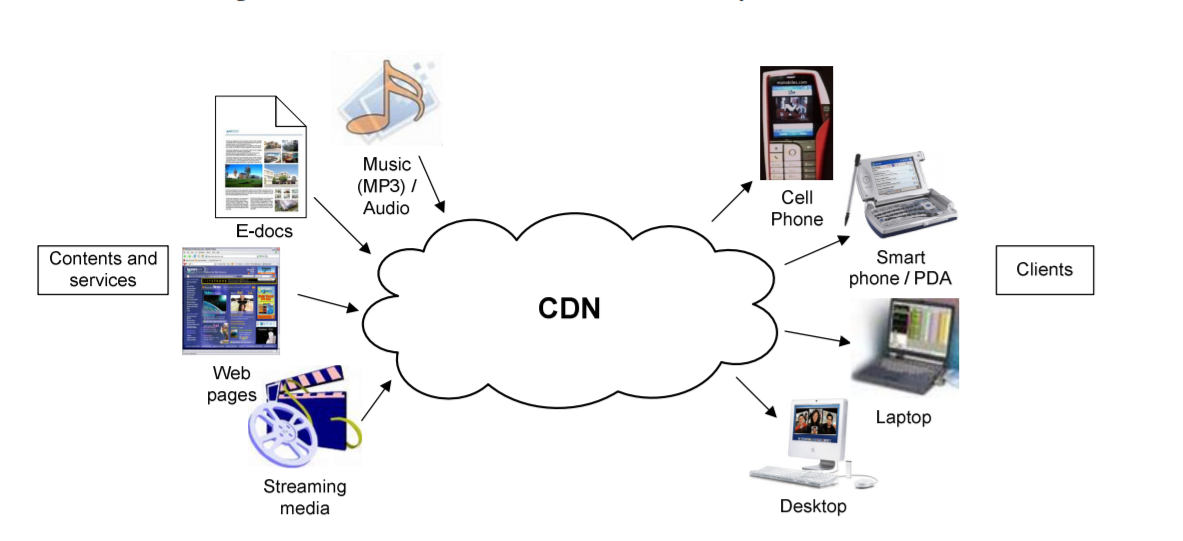
\includegraphics[height=7cm]{Figuras/contextualizacao.png} 
\label{figura:contextualizacao} 
\end{figure}
Temos v\'arios servi\c{c}os que se utiliza no dia a dia onde essa no\c{c}\~ao de CDN \'e completamente abstrata ao usu\'ario final. Como servi\c{c}os de Video-On-Demand de empresas de TV, spotify, Amazon Prime Video e at\'e Netflix, como \'e mostrado no artigo do \cite{adhikari2012unreeling}.
\newline
Existem hoje diversas empresas que fornecem esse servi\c{c}o ao redor do globo. Como:
\begin{itemize}
\item Akamai;
\item Limelight;
\item Level 3;
\item e etc.
\end{itemize}

Essas tr\^es redes s\~ao hoje, as principais fornecedoras de servi\c{c}o de CDN da Netflix. Cada um com um caracter\'istica e voltado pra um p\'ublico.
\subsection{AKAMAI}
\paragraph{Origem}- Massachusetts Institute of Technology (MIT), em 1995, com Tim Berners-Lee.
\paragraph{Pontos de atua\c{c}\~ao}
\begin{figure}[H]
\caption{Rede de distribui\c{c}\~ao Akamai}
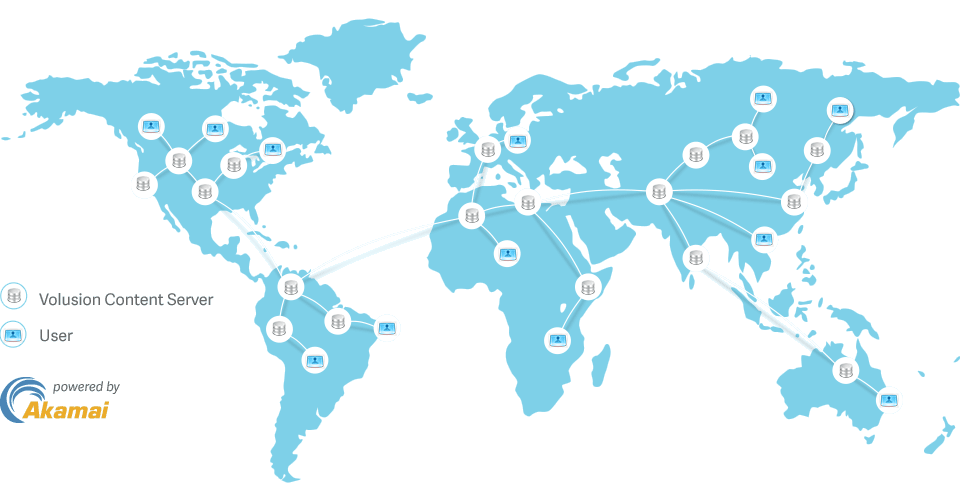
\includegraphics[width=12cm]{Figuras/akamai_map.png} 
\label{figura:akamai_map}
\end{figure}
\paragraph{Principais clientes}- Adobe, Airbnb, American Idol, Audi, Autodesk, EMC2, e muitas outras.
\subsection{Limelight}
\paragraph{Origem}- Tempe, Arizona, EUA.
\paragraph{Pontos de atua\c{c}\~ao}
\begin{figure}[H]
\caption{Rede de distribui\c{c}\~ao Limelight}
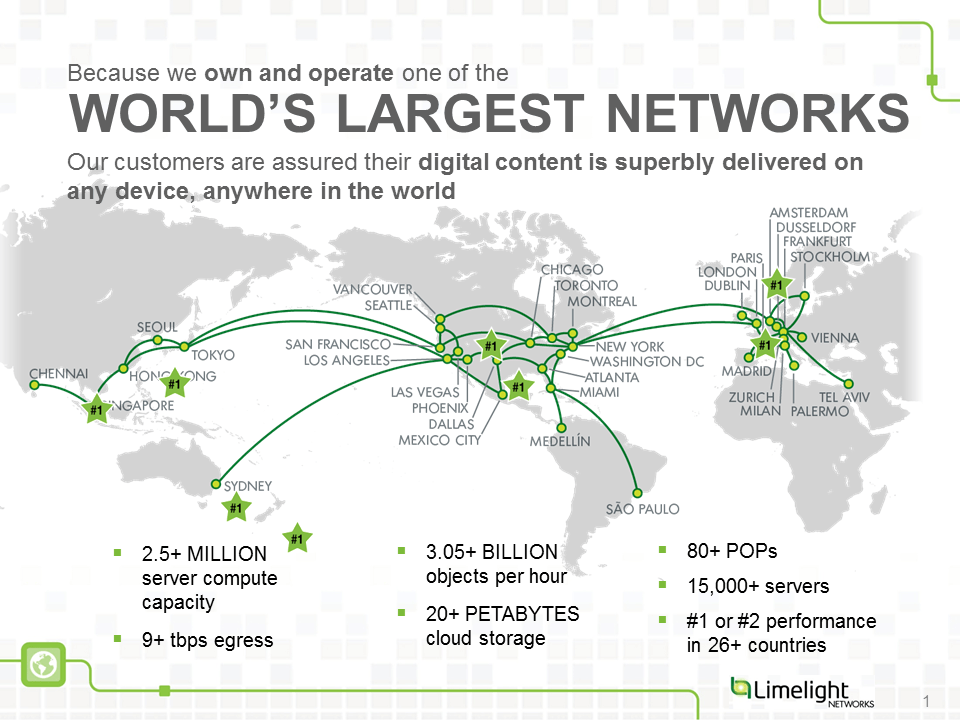
\includegraphics[width=12cm]{Figuras/limelight_map.png} 
\label{figura:limelight_map}
\end{figure}
\paragraph{Principais clientes}- N\~ao informado.
\subsection{Level 3}
\paragraph{Origem}- Monroe, Luisiana, EUA. 
\paragraph{Pontos de atua\c{c}\~ao}
\begin{figure}[H]
\caption{Rede de distribui\c{c}\~ao Level 3}
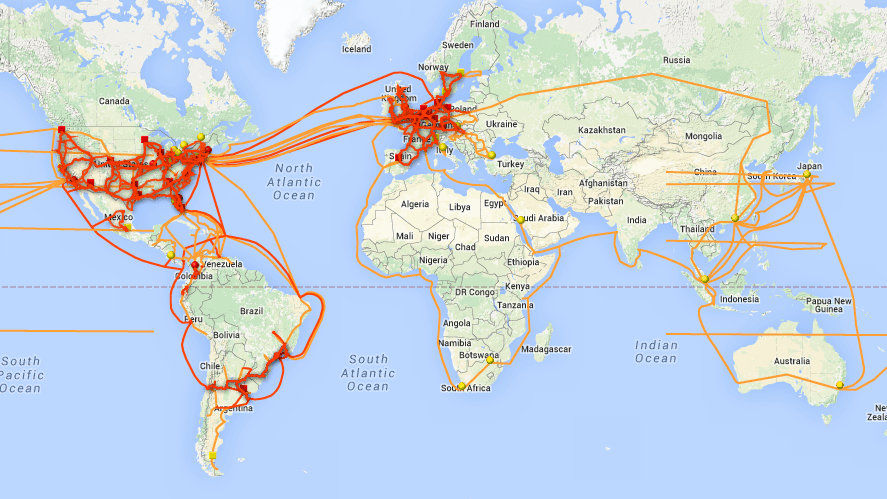
\includegraphics[width=12cm]{Figuras/level3_map.png} 
\label{figura:level3_map}
\end{figure}
\paragraph{Principais clientes}- N\~ao informado.
\subsection{Vis\~ao geral}
Todas essas redes se concentram praticamente no mesmo ponto. \'E claro, movida por uma quest\~ao financeira, todas elas est\~ao basicamente concentradas nos Estados Unidos, Europa e algumas adentram at\'e o mercado asi\'atico.
\newline
Nesse artigo vamos tentar entender um pouco mais a respeito de CDNs e tamb\'em um pouco do seu sistema de seguran\c{c}a. Sendo assim, poderemos dividir o restante desse artigo em duas partes: A primeira ser\'a relacionada somente a composi\c{c}\~ao da CDN, ou seja, tudo aquilo que \'e necess\'ario para se constituir uma CDN. Na segunda etapa falaremos primeiro um pouco sobre seguran\c{c}a em um \^ambito geral e depois aprofundaremos em seus conceitos voltados para CDN.